% !TeX spellcheck = en_US
% TODO: Finetune floats

\chapter{General Introduction and Objectives}
\label{ch:intro}

\section{Plastics in Agriculture}

The use of plastics in agriculture has grown exponentially in recent years \citep{MormileWorld2017}.
Between \numrange[range-phrase={ and }]{2013}{2019}, for example, the German agricultural sector consumed about \SI{1.1}{\mega\tonne} of plastics per year. This is equivalent to \SI{4.6}{\percent} of Germany's annual plastic consumption \citep{BertlingKunststoffe2021}. The majority of the agricultural plastics applied (\SI{50}{\percent}) is estimated to be films, fleeces, and nets used for greenhouse and low tunnels, complete field coverage, near-ground mulching\sidenote{See also Chapter~\ref{ch:plastic-mulching}.}, or silage storage \citep{MormileWorld2017,BertlingKunststoffe2021}.
Further applications are irrigation pipes, seed coatings, and plastic pots \citep{BertlingKunststoffe2021}. \Ac{pe} and \ac{pp} are by far the most used polymers, followed by \ac{ps}, \ac{pvc}, and \ac{pet} \citep{PlasticsEuropePlastics2019,ZhangNonbiodegradable2021}. In addition to that, agricultural landscapes receive mixed plastic inputs from sewage sludge and compost applications, littering, and erosion \citep{HurleyFate2018,BlasingPlastics2018,StubbinsPlastics2021}. All this makes agricultural land a particular hotspot for plastic debris \citep{CorradiniMicroplastics2021,ZhangNonbiodegradable2021} but also challenges the quantitative discrimination of the different sources of plastic inputs to agricultural soil.

Current estimates suggest that lost agricultural plastic covers account for annual plastic emissions of \SIrange{4}{9}{\kilo\gram\per\hectare} to agricultural landscapes in Germany. However, estimate errors are as high as \SI{+-100}{\percent} \citep{BertlingKunststoffe2021}. Moreover, empirical data on the fate of these losses remain largely missing. This includes the potential disintegration of lost plastics into smaller debris and their distribution and incorporation into the soil environment. The knowledge gap is probably attributed to the analytical challenges the soil matrix poses for a reliable plastic quantification \citep{QiBehavior2020}. In this regard, novel thermoanalytical approaches may be particularly promising.

\section{Thermoanalytical Methods for Plastic Characterization and Quantification}

Thermoanalytical methods such as \ac{dsc} or \ac{ega} are commonly applied in polymer science to study the material properties of a sample while subjected to temperature changes. \Ac{dsc}, for instance, monitors the amount of energy required to change the temperature of a sample. The technique is used to determine the melting, crystallization, and glass transition temperatures of a polymer \citep{MenczelDifferential2009}. These parameters are informative proxies for characterizing and better understanding the polymer's (supra)molecular structure and morphology including its molecular weight and degree of cross-linking \citep{BialeSystematic2021}. The exposure of plastics to \ac{uv} light, water, or temperature changes, for instance, causes scissions in the polymer backbone, carbonyl formation, and volatilization of oligomers and polymer additives. Such changes are typically summarized as aging and often lead to embrittlement and eventual disintegration of plastics \citep{VolynskiiStructural2007,WhitePolymer2006}. \Ac{dsc} can thus help to scrutinize the disintegration potential of a plastic material into smaller debris.

\begin{margintable}
	\centering\footnotesize
	\caption[Decomposition temperatures of selected polymers.]{Decomposition temperatures of selected polymers \citep{BeylerThermal2002,FerriolThermal2003,ShionoThermoanalytical2015}.}\label{tab:polymer-decomposition}
	\begin{tabular}{lS[table-format = 3]S[table-format = 3]}
		\toprule
		{Polymer} & {Onset\textsuperscript{\textdaggerdbl}} & {Peak maximum} \\
		& [\si{\degreeCelsius}] & [\si{\degreeCelsius}] \\
		\midrule
		\acs{ldpe} & 318 & 490 \\
		\acs{hdpe} & 275 & \\
		\acs{pp} & 315 & 466 \\
		\acs{ps} & 330 & 441 \\
		\acs{pmma} & 282 & 377 \\
		\acs{pvc} & 184 & 320 \\
		\acs{ptfe} & 502 & 579 \\
		\bottomrule
		\multicolumn{3}{p{.9\linewidth}}{\textsuperscript{\textdaggerdbl}temperature at which \SI{1}{\percent} of polymer mass loss occurred in an \ch{N2} atmosphere; \acs{ldpe} = \acl{ldpe}; \acs{hdpe} = \acl{hdpe}; \acs{pp} = \acl{pp} (isotactic); \acs{ps} = \acl{ps}; \acs{pmma} = \acl{pmma}; \acs{pvc} = \acl{pvc}; \acs{ptfe} = \acl{ptfe}.} \\
	\end{tabular}
\end{margintable}

\Ac{ega} enables the identification and quantification of gases evolving from a sample at a specific temperature or temperature range using \iac{ms} or \ac{ftir} detector. If coupled with a microbalance, the weight loss of the sample can be recorded simultaneously. This setup is called \ac{tga-ms} \citep{PrimeThermogravimetric2009}. \Ac{py-gc-ms} adds the possibility of chromatographically separating the evolved gases prior to detection \citep{Rial-OteroReview2009}. 
Depending on the applied temperature, the main processes leading to gas evolution are thermodesorption and decomposition. Which process prevails at what temperature range depends on the type of sample. The release of volatile additives like plasticizers, slip agents, or antioxidants is typically studied between \SIrange[range-phrase = { and }]{100}{300}{\degreeCelsius} \citep{ReichelSystematic2020,AkouesonIdentification2021}. Polymer decomposition sets in above \SI{180}{\degreeCelsius} and peaks at \SIrange{300}{600}{\degreeCelsius} (Table~\ref{tab:polymer-decomposition}). If the polymer is decomposed in an inert or reductive atmosphere like \ch{N2} or \ch{H2}, the process is called pyrolysis \citep{BeylerThermal2002}.

\begin{marginfigure}[\baselineskip]
	\centering
	\schemestart
	\chemname[1.5\baselineskip]{\chemfig{-[@{op,.5}::30]-[::-60]-[@{cl,0.5}::60]}
\polymerdelim[delimiters ={[]}, height = 1.5em, depth = 1.5em, indice = n]{op}{cl}}{\Acf{pe}}
	\arrow{0}[-90,0.5]
	\chemname[1.5\baselineskip]{\schemestart
\chemname[1.5\baselineskip]{
	\chemfig{-[@{op,.5}::30](-[::60,0.8])-[::-60]-[@{cl,0.5}::60]}
	\polymerdelim[delimiters ={[]}, height = 3.5em, depth = 1.5em, indice = n]{op}{cl}
	}{\Acf{pp}}
\arrow{->[ $\Delta$T ]}[,1.5]
\subscheme{
	\chemname[1.5\baselineskip]{
		\chemfig{-[::30]-[::-60]-[::60]-[::-60]}
	}{$n$-pentane}
	\arrow{0}[,.0]
	\+
	\arrow{0}[,.0]
	\chemname[1.5\baselineskip]{
		\chemfig{=[::30](-[::60,0.8])-[@{op,.5}::-60]-[::60](-[::60,0.8])-[@{cl,0.5}::-60]-[::60]-[::-60]}
		\polymerdelim[delimiters ={[]}, height = 3.5em, depth = 1.5em, indice = x]{op}{cl}
	}{methylalkenes}
}
\schemestop}{\Acf{pp}}
	\arrow{0}[-90,0.5]
	\chemname[1.5\baselineskip]{\chemfig{-[@{op,.1}::30,1.1](-[::60,0.8]*6([::0,0.8]-=-=-=-))-[::-60]-[@{cl,0.5}::60]}
\polymerdelim[delimiters ={[]}, height = 8em, depth = 1em, indice = n]{op}{cl}}{\Acf{ps}}
	\arrow{0}[-90,0.5]
	\chemname[1.5\baselineskip]{\chemfig{
	[,0.8]O=[:60]
	(-[:120]O-[@{op,.5}:180])
	-*6([::0]-=-
	(-(-[:300]O--[:-60]-[@{cl,0.5}])=[:60]O)
	=-=-)
}
\polymerdelim[delimiters ={[]}, height = 1em, depth = 6.5em, indice = n]{op}{cl}}{\Acf{pet}}
	\schemestop
	\vspace{\baselineskip}
	\caption[Structural formulas of the polymers investigated in this thesis.]{Structural formulas of the polymers investigated in this thesis; see \citet{IvlevaChemical2021} for details.}
	\label{fig:polymers}
\end{marginfigure}

Pyrolytic reactions typically involve the random, homolytic cleavage of the polymer backbone into oligomer radicals. A consecutive hydrogen transfer, $\beta$-scission, or radical recombination produces stable monomers, oligomers, or derivatives thereof \citep{BockhornKinetic1999,BeylerThermal2002}. The pyrolysis of \ac{pe} (Figure~\ref{fig:polymers}), for instance, produces $n$-alkanes, $n$-alkenes, and $n$-alkadienes of different chain lengths as major pyrolysates. \Ac{pp} decomposes into $n$-pentane and various methylalkenes including 2,4-dimethyl-1-heptene. Pyrolyzing \Ac{ps} mainly yields the styrene monomer, dimer, and trimer, as well as toluene and $\alpha$-methylstyrene. \Ac{pet} decomposes into 4-(vinyloxycarbonyl) benzoic acid monomers, respective dimers and trimers, benzoic acid, and \ch{CO2} \citep{TsugePyrolysis2011}\sidenote{See Table~\ref{tab:py-products} for a detailed overview of pyrolysis products.}.

Quantitative \ac{tga-ms} or \ac{py-gc-ms} applications aim to identify pyrolysates that can be used as characteristic markers for polymer quantification. At the same time, these marker compounds should not occur in the analyzed soil matrix. To avoid interferences, both instrumental analytics and sample preparation need to be carefully adjusted.

\section{Soil---A Complex Analytical Matrix}
\label{sec:intro:soil-matrix}

Soil is a multiphased, heterogeneous mixture of solids, liquids, and gases. The solid phase consists of various minerals and \ac{som} aggregated to a porous system that is filled with soil air and soil solution. The soil composition depends on the parent rock and its weathering, past and present land use, the vegetation, and climate \citep{BrummerIntroduction2016}. 

Soil minerals are classified by size into sand (\SI{63}{\micro\meter} to \SI{2}{\milli\meter}), silt (\SIrange{2}{63}{\micro\meter}), and clay (\SI{<2}{\micro\meter}) \citep{SponagelBodenkundliche2005}. They mainly consist of silica (\ch{SiO2}) but may also contain alumina (\ch{Al2O3}) and other potassium, sodium, calcium, iron, or manganese oxides. Clay minerals can be further grouped into kaolinites, smectites, vermiculites\slash illites, and chlorites dependent on the silica structure and surface charge. The surface charge is typically negative and balanced with potassium, sodium, or other divalent ions \citep{StahrInorganic2016}.

\Ac{som} comprises plant and animal litter at various stages of decomposition. The labile \ac{som} fraction
contains easily-degradable molecules like peptides, (phospho)lipids, and carbohydrates (Figure~\ref{fig:som-groups}), whereas the stable, humic fraction consists of more complex macromolecules. Such macromolecules may originate from lignin or other natural polymers like chitin or cellulose \citep{Kogel-KnabnerSoil2016}.
The amphiphilic domains of the \ac{som} constituents may interact with clay minerals and aluminum or iron oxides via electrostatic interactions or Van der Waals forces forming organo--mineral complexes \citep{KleberConceptual2007}.

The environmental analysis of specific target compounds like \ac{pe} or \ac{pp}, namely the analytes, typically requires a certain degree of sample preparation prior to their quantification. Ideally, such a procedure removes a large part of the sample matrix while preserving or even enriching the analytes. This not only increases the sensitivity of the method but reduces potential interferences from matrix constituents. Separating the matrix from the analytes usually exploits differences in their physicochemical properties like their density, their specific interaction with other solid or liquid phases, or their recalcitrance towards acids, bases, or oxidation agents\sidenote{See Chapter~\ref{ch:analytical-techniques} for details.}. The more similar the analyte and the matrix are, the harder becomes their separation.

\begin{margintable}
	\centering\footnotesize
	\caption[Solubility characteristics of selected polymers.]{Solubility characteristics of selected polymers \citep{BivensPolymertoSolvent2016}.}\label{tab:polymer-dissolution}
	\begin{tabular}{llS[table-format = 3]}
		\toprule
		{Polymer} & {Solvent} & {Temperature} \\
		&  & [\si{\degreeCelsius}] \\
		\midrule
		\acs{pe} & \acs{tcb} & 160 \\
		\acs{pp} & \acs{tcb} & 160 \\
		\acs{ps} & \acs{thf} & 40 \\
		\acs{pmma} & \acs{thf} & 35 \\
		\acs{pvc} & \acs{thf} & 25 \\
		\bottomrule
		\multicolumn{3}{p{.9\linewidth}}{\acs{tcb} = \acl{tcb}; \acs{thf} = \acl{thf}.} \\
	\end{tabular}
\end{margintable}

In this respect, soil is a particularly challenging matrix for its heterogeneous, multiphased nature. Separating plastic debris from soil is even more complex as both are particulate phases of polymeric composition \citep{StubbinsPlastics2021,SchaumannSoil2006}. This could be plastic particles that are coated with natural polymers or occluded in soil aggregates. 
Plastic quantification is further complicated when soil constituents and polymers cause identical or equivocal signals during the measurement process. Such interferences currently affect the majority of microspectroscopic and thermoanalytical methods for the analysis of plastic debris in environmental samples. Microspectroscopic methods only deliver particle-based information and are prone to interferences from \ac{som} autofluorescence or physical obstruction of plastic particles with soil constituents. On the contrary, mass-based, thermoanalytical methods may suffer from the structural similarities between polymers (Figure~\ref{fig:polymers}) and \ac{som} constituents (Figure~\ref{fig:som-groups}) leading to identical pyrolysates like $n$-alkanes or styrene\sidenote{See Chapter~\ref{ch:analytical-techniques} for a more comprehensive method comparison.}.

This may be overcome with a well-designed analytical approach which, for instance, exploits the selective solubility of certain polymers in a specific organic solvent at elevated temperature without co-dissolving interfering matrix constituents like \ac{som}. Dissolving polymers is common practice for the analysis of polymer molecular weights via \ac{sec} and \ac{gpc} (Table~\ref{tab:polymer-dissolution}) but may as well be combined with thermoanalytical methods\sidenote{See Chapter~\ref{ch:analytical-techniques} for details.}.

\begin{figure*}
	\centering
	\footnotesize
	\schemestart
	\chemname[\baselineskip]{% iso 17:0
\definesubmol{i17:0}{
	-[:30]
	(
	-[:90]
	)
	-[:330]
	-[:30]
	-[:330]
	-[:30]
	-[:330]
	-[:30]
	-[:330]
	-[:30]
	-[:330]
	-[:30]
	-[:330]
	-[:30]
	-[:330]
	-[:30]
	(=[:90]O)
	-[:330,,,1]O
}

\definesubmol{turned-i17:0}{
	O
	-[:-150](=[:-90]O)
	-[::-60]
	-[::60]
	-[::-60]
	-[::60]
	-[::-60]
	-[::60]
	-[::-60]
	-[::60]
	-[::-60]
	-[::60]
	-[::-60]
	-[::60]
	-[::-60]
	-[::60](-[:-90])
	-[::-60]
}

% Merge to phospolipid
\chemfig{!{i17:0}-[:-75](-[:45])(-[:-30]-[::60]O-[::-60]P(-[:90]O)(-[:0]O^{-})=[:-90]O)-[::-75]-[::-75]!{turned-i17:0}}}{(Phospho)lipids}
	\arrow{0}[-90,0.5]
	\chemname[\baselineskip]{% N-acetylglucosamine
\definesubmol{GlcNAc}{
	O-[:10,.7]
	(
	-[:-10](-[:150,0.7]-[2,0.7]OH)
	-[:10]{O}-[:-50]
	)
	-[:-50](-[:170]HO)
	-[:10](-[:-55,0.7]NH([::-90,.7]-([::60]-)=[::-60]O))
	-[:-10]
	-[:10,.7]O
}

% Turned N-acetylglucosamine
\definesubmol{turned-GlcNAc}{
	-[:-10,.7]
	(
	-[:10](-[:-150,0.7]-[6,0.7]OH)
	-[:-10]{O}-[:50]
	)
	-[:50](-[:-170]HO)
	-[:-10](-[:55,0.7]NH([::90,.7]-([::-60]-)=[::60]O))
	-[:10]()
	-[:-10,.7]
}
	
% Merge to chitin
\chemfig{-[@{op,.5}:-10,.7]!{GlcNAc}!{turned-GlcNAc}-[@{cl,0}:-10,.25]}
\polymerdelim[delimiters ={[]}, height = 3em, depth = 3em, indice = n]{op}{cl}}{Polycarbohydrates (here chitin)}
	\arrow{0}[-90,0.5]
	\subscheme{
		\chemname[\baselineskip]{% Serine, Phenylalanine, Glycine, Proline
\schemestart
\chemname[\baselineskip]{
	\chemfig{
		H_2N-[:-30](-[:30]-[:-30]OH)-[:-90](=[:-150]O)-[:-30]NH-[:-90](-[:-150]-[:-90]*6(-=-=-=))-[:-30](=[:30]O)-[:-90]NH-[:-30](-[:30]-[:-30]SH)-[:-90](=[:-150]O)-[:-30]NH-[:-90]-[:-150](=[:-90]O)-[:150]O^{-}
	}
}{Peptides}
\arrow{->[ $\Delta$T ]}[,1.5]
\subscheme{
	\chemname*[\baselineskip]{
		\chemfig{
			=^[:180]-[:252,,,2]HN-[:324,,2]=^[:36](
			-[:108]
			)
		}
	}{pyrrole}
	\arrow{0}[,0]
	\+
	\arrow{0}[,0]
	\chemname*[\baselineskip]{
		\chemfig{
			=^[:270]-[:330]
			=^[:30]-[:90](
			=^[:150]-[:210]
			)
			-[:18]=_[:306]-[:234]{N}{H}(
			-[:162]
			)
		}
	}{indole}
	\arrow{0}[,0]
	\+
	\arrow{0}[,0.1]
	\ldots
}
\schemestop}{Peptides}
		\arrow{0}[,1.5]
		\chemname*[\baselineskip]{\chemfig{[:-60]*6(=(--[::-60](-[:90]O^{-})(=O))-*6(-(-)=-(--[:-90]OH)=-)=-(--[::-60]-)=(-(-[:150]O^{-})([:30]=O))-)}}{Aromatic lignin derivatives}
	}
	\schemestop
	\vspace{\baselineskip}
	\caption[Common \acs{som} groups.]{Common \acf{som} groups \citep{NewcombDeveloping2017,Kogel-KnabnerSoil2016}.}
	\label{fig:som-groups}
\end{figure*}

\section{Objectives and Outline of this Thesis}
\label{sec:intro:objectives}

Driven by the increasing, yet virtually unquestioned application of agricultural plastic covers, my thesis begins with a critical evaluation of the scientific knowledge on the benefits and potential risks of agricultural plastic covers to the soil environment (Chapter~\ref{ch:plastic-mulching}, Figure~\ref{fig:thesis-overview}). I hypothesize that agricultural plastic covers unintentionally left in the field fragment to plastic debris smaller than \SIrange{1}{5}{mm}, called microplastics \citep{HartmannAre2019}; meaning that agricultural plastic covers function as a source of plastic debris in soil.
However, robust analytical tools for plastic quantification in soil matrices were still missing at that stage. Prior to addressing my hypothesis, I thus developed and tested new methods for the quantitative analysis of plastic debris in soil. This method development included the following objectives:

\begin{enumerate}
	\item\label{en:thermoanalysis} Assessing the applicability of thermoanalytical methods for the mass-based quantification of plastic debris in soil.
	\item\label{en:chromatography} Making use of additional chromatographic separation to increase the selectivity of the method for polymer mixtures.
	\item\label{en:dissolution} Minimizing matrix interferences and increasing sample homogeneity by dissolving the polymer analytes in an organic solvent prior to quantification.
	\item\label{en:application} Applying the final method in a first screening study of agricultural soil covered with plastic.
\end{enumerate}

\begin{figure*}
	\centering
	\label{fig:thesis-overview}
	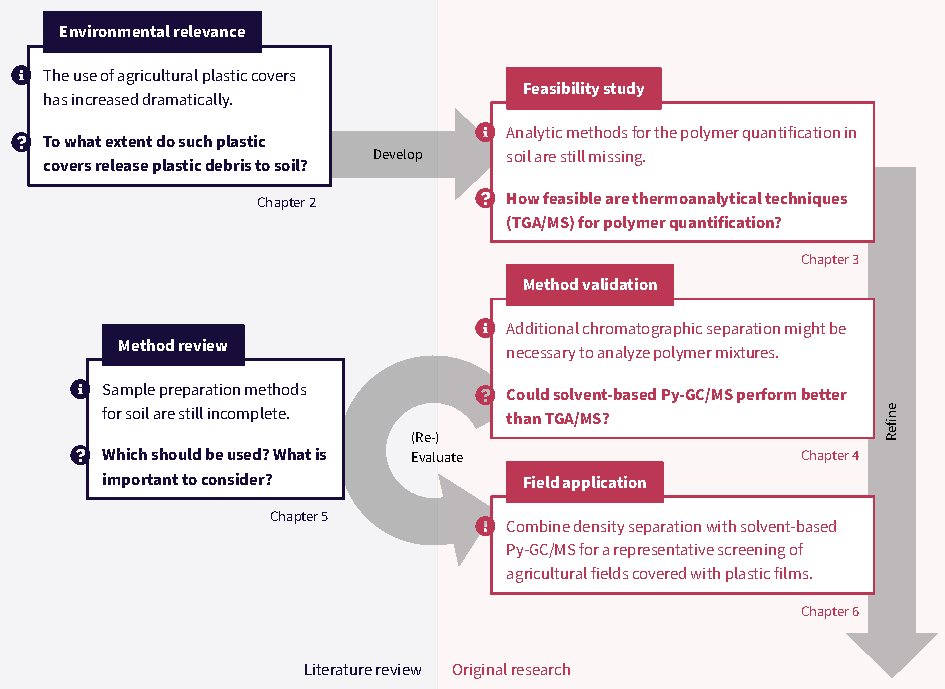
\includegraphics[width=\textwidth]{figures/thesis-overview}
	\caption{Conceptual overview and research questions addressed in this thesis.}
\end{figure*}

Objective \ref{en:thermoanalysis} is addressed in Chapter~\ref{ch:tga-ms-method}. This first proof-of-principle study relied on \ac{pet} as a model compound and one reference soil to investigate the potential of \ac{tga-ms} for plastic quantification. The method was designed to enable the direct analysis of \SI{50}{\milli\gram} soil without any sample preparation. To facilitate the analysis of polymer mixtures and increase instrumental sensitivity, I continued method development using \ac{py-gc-ms} (objective \ref{en:chromatography}). However, \ac{py-gc-ms} is typically restricted to sample amounts \SI{<1}{\milli\gram} which poses high requirements on sample homogeneity. To overcome this and to reduce the risk of potential matrix interferences, I used \ac{tcb} to selectively dissolve \ac{pe}, \ac{pp}, and \ac{ps} in three different reference soils (objective \ref{en:dissolution}). This new solvent-based \ac{py-gc-ms} approach made up to \SI{4}{g} soil amenable to the quantification of plastic debris (Chapter~\ref{ch:py-gc-ms-method}). Chapter~\ref{ch:analytical-techniques} critically (re-)evaluates this and other analytical techniques. With this knowledge at hand, I further refined my method. This involved adjustments in the extraction mixture to increase polymer solubility and the addition of a suitable yet simple sample preparation technique to the existing \ac{py-gc-ms} approach. Thereby, plastic debris could be quantified from \SI{50}{g} of soil. This sample amount was considered sufficiently large for a representative screening study of eight agricultural field covered with plastic films (objective~\ref{en:application}, Chapter~\ref{ch:screening}). Therein and in the following general discussion (Chapter~\ref{ch:general-discussion}) I conclusively address the key hypothesis of this thesis and reflect on the implications of my findings.
